\chapter{Implementation details}


For this purpose, highly customizable workflows based on PyTorch have been implemented.


Furthermore, some basic notions which are of particular importance for the performance of the architectures, e.g. norm layers, will be explained in some more detail.

Furthermore, 'molecules' with less than two atoms were discarded. (Certainly, this does not make any difference because usually in the datasets there are only proper molecules; however, in some cases, defective SMILES led to such entries.) 

So in a first step, for multiple datasets (see tasks, datasets) provisional results were computed and it was checked whether significant differences between approaches and architectures can be found.

For most architectures and parameter settings, the first benchmarks were performed using the simple, often used ESOL dataset. Given the results on this dataset, selected methods were investigated in more detail on other datasets.

If not stated otherwise, the datasets were not preprocessed, e.g. no outliers or duplicates were removed.



higher-order

The evaluation of such a network architecture is also interesting for comparison purposes since they were not tested on molecular graphs except for the ZINC dataset in the Nested GNN publication (In the format of the default ZINC loader from Pytorch Geometric with solely the atom type as atom feature).

The only used feature was the atom type.
(In the format of the default ZINC loader from Pytorch Geometric). (In principle, it should be easy to project lists of features to 1D.)


In this regard, one would also have to reflect what constitutes a fair comparison: For GNNs – given sufficient input data as well as neuron and layer numbers -, it is rather natural that additional information, e.g. additional node features, increase the performance (as long as it is really additional information about the underlying distribution and not just noise).



\subsection{Further implementation details}

On several occasions, this required the implementation of the models with different libraries.
In particular, additional runs can be started and, upon completion, will be automatically added to the analysis pipeline.
Either optuna hyperoptimization is performed and subsequently a run with the optimized parameters is performed, or manually set parameters can be used.
Additionally, it was also implemented to use other classifiers for the fingerprints as DNNs, e.g. SVMs and Gradient Boost methods like LightGBM.

For optimization a multi-step approach was chosen: Given the amount of data sets, splits, parameters, architectures and possible feature combinations, it would be infeasible to run hyperparameter optimization for every reasonable setting.
In a first step, for all datasets hyperparameter optimization for the models of main interest (GCN, GIN, Morgan fingerprint with bitwise- and count-features and, for some some datasets, Neural Fingerprint) was performed with default settings (for instance, the default atom and bond features) and deactivation of additional, possibly performance-increasing architectural features like normalization and dropout layers.

Afterwards, the optimal hyperparameters determined have been used for extended experiments, for instance using different atom features or jumping knowledge.

In cases of promising results - i.e. when without new determination of optimal hyperparameters the results were better, e.g., in terms of mean error or variance of the error -, hyperparameter optimization was performed anew for these settings.

Unfortunately, for these classification tasks in almost none publication it is revealed how this data imbalance is tackled (which suggests that the data is taken as it is). Given the fact that most typical benchmark datasets (e.g. from MoleculeNet) are highly imbalanced, this is very problematic. It turns out to be even more severe since many split techniques, e.g. the usually, in addition to the random split, applied scaffold split, leverages the imbalancing extremely.
Common ways of treating imbalanced datasets are upsampling, i.e. instances of the rare class are copied, and weighting, i.e. the errors/losses get weighted proportional to their frequency in the dataset.



\subsection{Data splits}

Alternatively to random splitting, one can apply scaffold splitting \cite{Bemis.1996}.
The assumptions of the reasoning behind the scaffold split are not always met: Firstly, it could be…
On the other hand, it could be that a totally different mechanism is responsible for activity or toxicity in another compound; it is obvious that such generalization can be extremely difficult or even impossible. 

Scaffold splitting explores the difficulties of predictors in dealing with inter-scaffold generalization, whereas activity cliff prediction affords intra-scaffold generalization. \cite{Deng.2023}

A straightforward idea for splitting is to directly use similarity information, e.g. obtained by Tanimoto similarity.


Given the high correlation between molecular weight and a multitude of properties, e.g. solubility, such a weight split often also entails a split with regard to the objective value.
It should be noted that the MolecularWeightSplitter of the DeepChem- and of the DGL-library are fully deterministic and does not depend on the ordering of the input data, i.e. shuffling does not change the output of the splitter. 

The DeepChem TaskSplitter tries to split the datasets as evenly as possible with regard to the objective value (i.e., for classification tasks, the proportion of all sets generated by the split should be as equal to the original input as possible, and for regression tasks, the same holds for the distribution of the values to be predicted).

The DGL SingleTaskStratifiedSplitter can also be used.


Given the main difference between the Graph representations and the fixed-size fingerprints, namely that the former can specify due to their learnable weights to a specific task, the results for the Task splitting, in which splitting is done so that batches with a similar objective value are in the same set, are of special interest since it requires extrapolation with respect to the target value.

For Task splitting, patches of a specific size are selected.

Furthermore, splitting techniques which do not use discrete patches, but allow an overlap between the distributions by sampling from a Gaussian distribution (of course, other choices would be possible) have been implemented.

Fingerprint- and MinMax-Splitters are also implemented in the DeepChem-Library. The Fingerprint-Splitter sequentially adds molecules to one of the sets; it checks which molecule is least similar to all others in the sets and adds it to the opposite set. Similarly, the MinMax-Splitter constructs a test set which is as diverse as possible. 

Butina splitting which creates clusters based on Tanimoto similarity. \cite{Butina.1999}
(In the original publication, Butina splitting worked with Daylight fingerprints as input for the clustering algorithm, whereas the implementation in DeepChem uses bitwise Morgan Fingerprints created via RDKit.)

UMAP splitting was additionally implemented as a class for the DeepChem interface.
\cite{Guo.2024} reports that UMAP splitting provides much more difficult splits than the usual scaffold split. In \cite{Guo.2024}, the procedure was not described in details, but it seems that the approach from \cite{HernandezHernandez.2023} was adopted. The parameters for UMAP splitting were taken form this publication.
Again molecular fingerprints are computed, but afterwards applied to the UMAP dimensionality reduction. The low-dimensional representations are afterwards merged in batches using agglomerative clustering and appropriately assigned to the splits.

It should be noted that this approach involves some arbitrarily chosen parameters, e.g. the UMAP settings, the application of agglomerative clustering and the fingerprint itself.
A more thorough investigation of the effect of the clustering algorithm on the emerging splits and, in consequence, on performance evolution could be insightful.

It is not unlikely that depending on the type of split different hyperparameter combinations are optimal, since the effective task changes: For random splits, it is rather interpolation, whereas for scaffold splits, or other split techniques which minimize the similarity between training and validation/test set, the goal is extrapolation.
(It should be noted that also the amount of available data can lead to different optimal hyperparameter configurations.)

For the ESOL dataset, the effects of the splitting technique are shown in fig.


However, a fair evaluation of differences in variance between splitting techniques is even more difficult because depending on the technique, the similarity of the split sets is highly different and is also associated with the data (for instance, small datasets with a limited number of scaffolds will give very similar scaffold splits).


\subsection{Imbalanced data}


However, it should be noted that the usage of over-sampling methods which create synthetic data like SMOTE is potentially problematic in this context since it would probably tremendously exacerbate the danger of overfitting. (However, the analysis of the performance on such augmented datasets could be used for an investigation of the problem.)

Similarly to the more general question whether additional data can be harnessed by the models, in this respect the question is whether additional inactive compounds improve performance, i.e. it could be that they  lead to a reduction of false positives.

It should be noted that in most publications details how imbalanced data has been treated is missing. This is also true of performance benchmarks of the MoleculeNet datasets which nonetheless exhibit high imbalance and thus decisions like weighting of the rare class could definitely make a huge difference.


\subsection{Encoding of atom and edge features}


Table shows the features used by these in-built featurizers.

In the architectures which support edge information, the default edge featurizers from Pytorch Geometric and DGL are used. 

It should be noted that many of the edge features do not provide new information, but are redundant due to the atom features; however, this does not necessarily imply that this additional input has no impact on performance.

It could be insightful to test whether for feature sets without such a feature the optimal radius is different (one would it expect to be bigger).

\subsection{Classification of features}

Given the diverse origins - SMARTS strings, default featurizer of the ML libraries -, it seems convenient to distinguish several types of features:

1) features directly encompassing more distant atoms: the number of heavy neighbours falls into this category. Concerning the Morgan algorithm, it should be noted that the incorporation of this feature can bias results because indirectly there is always information of the next neighbour layer incorporated

2) features which only indirectly encompass more distant atoms: e.g., the property of aromaticity belongs to a specific atom, but it also tells more about the more distant neighbourhood, e.g. there have to be several further atoms in a bigger radius which participate in a ring and thus exhibit aromaticity.

3) features which indirectly encompass information of the bonding partners: many features provide information about the bonding to adjacent atoms, e.g. hybridization and the number of radical electrons

4) features solely dependent on the atom: atomic number / atomic weight, number of valence electrons, but also properties like electronegativity or the melting point of the element
The boundary between 2) and 3) is rather obscure, 4) however is clearly distinct from the other features.

Features of group 4) can be usually found in the periodic table and directly incorporate chemico-physical knowledge on the element level.

For the circular fingerprints, most of these additional features are redundant since they do not allow a better differentiation of structures. This is in particular true for group 4). (Usually the atomic number is provided as feature; since these features from the periodic table, like electronegativity, are in a unique mapping with the atomic number, they do not provide new information for the distinction of substructures.) In contrast, for the GNNs, the additional information can be harnessed for updating the weights according to the specific task or even learn general chemical insights.


\begin{table}
    \centering
    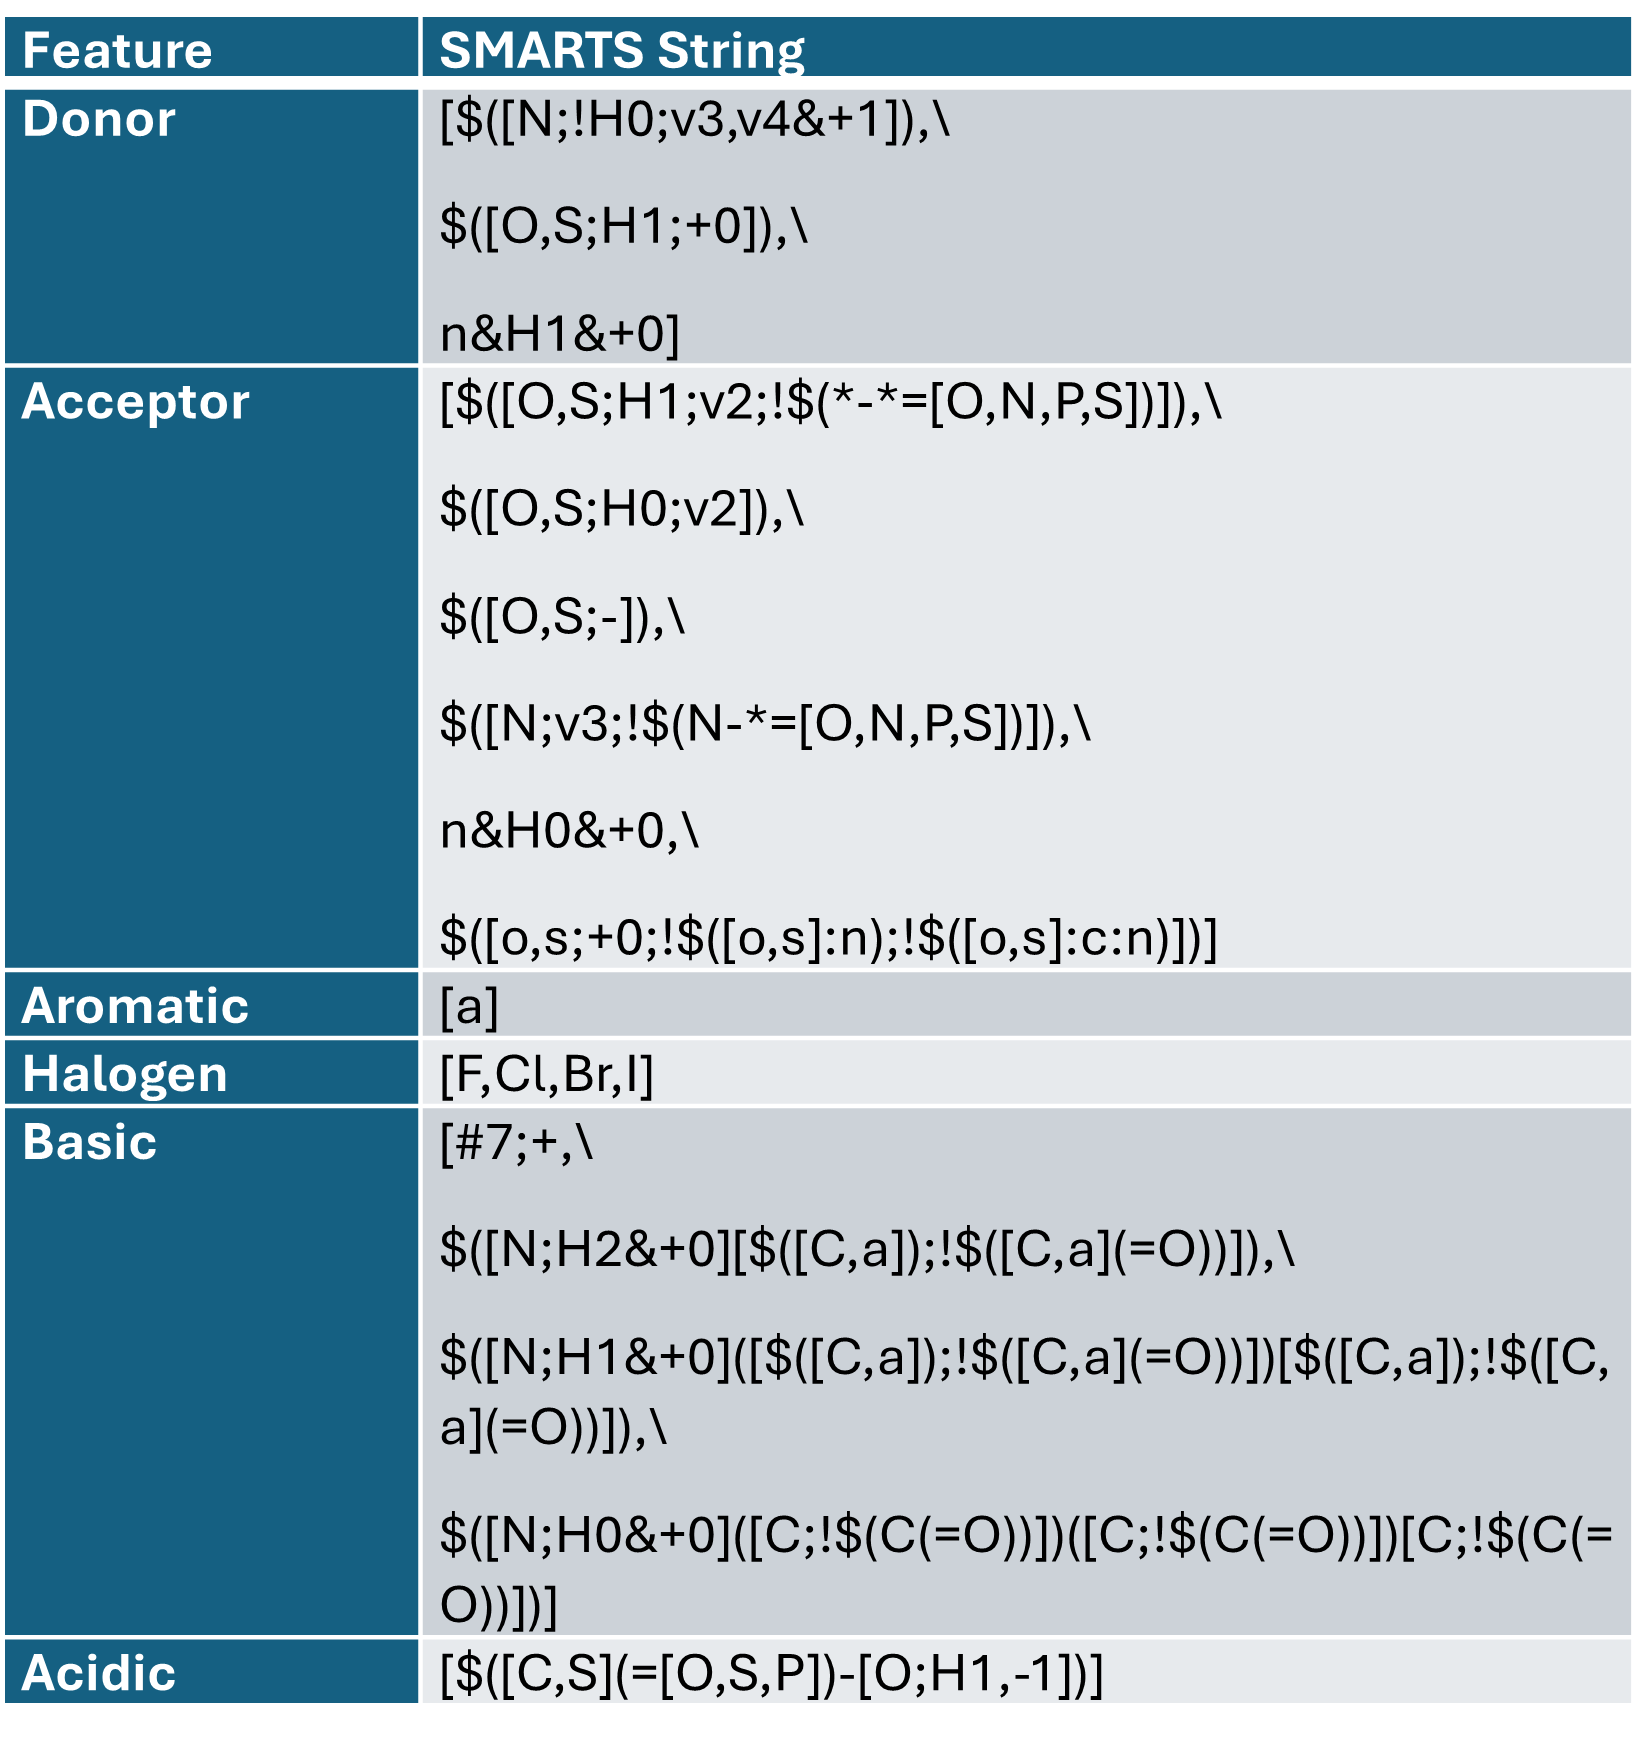
\includegraphics[width=0.8\linewidth]{rdkit_featurefp_features.png}
    \caption{Features used in the Morgan FeatureFP of RdKit}
    \label{tab:rdkit_featurefp_features}
\end{table}

\begin{table}
    \centering
    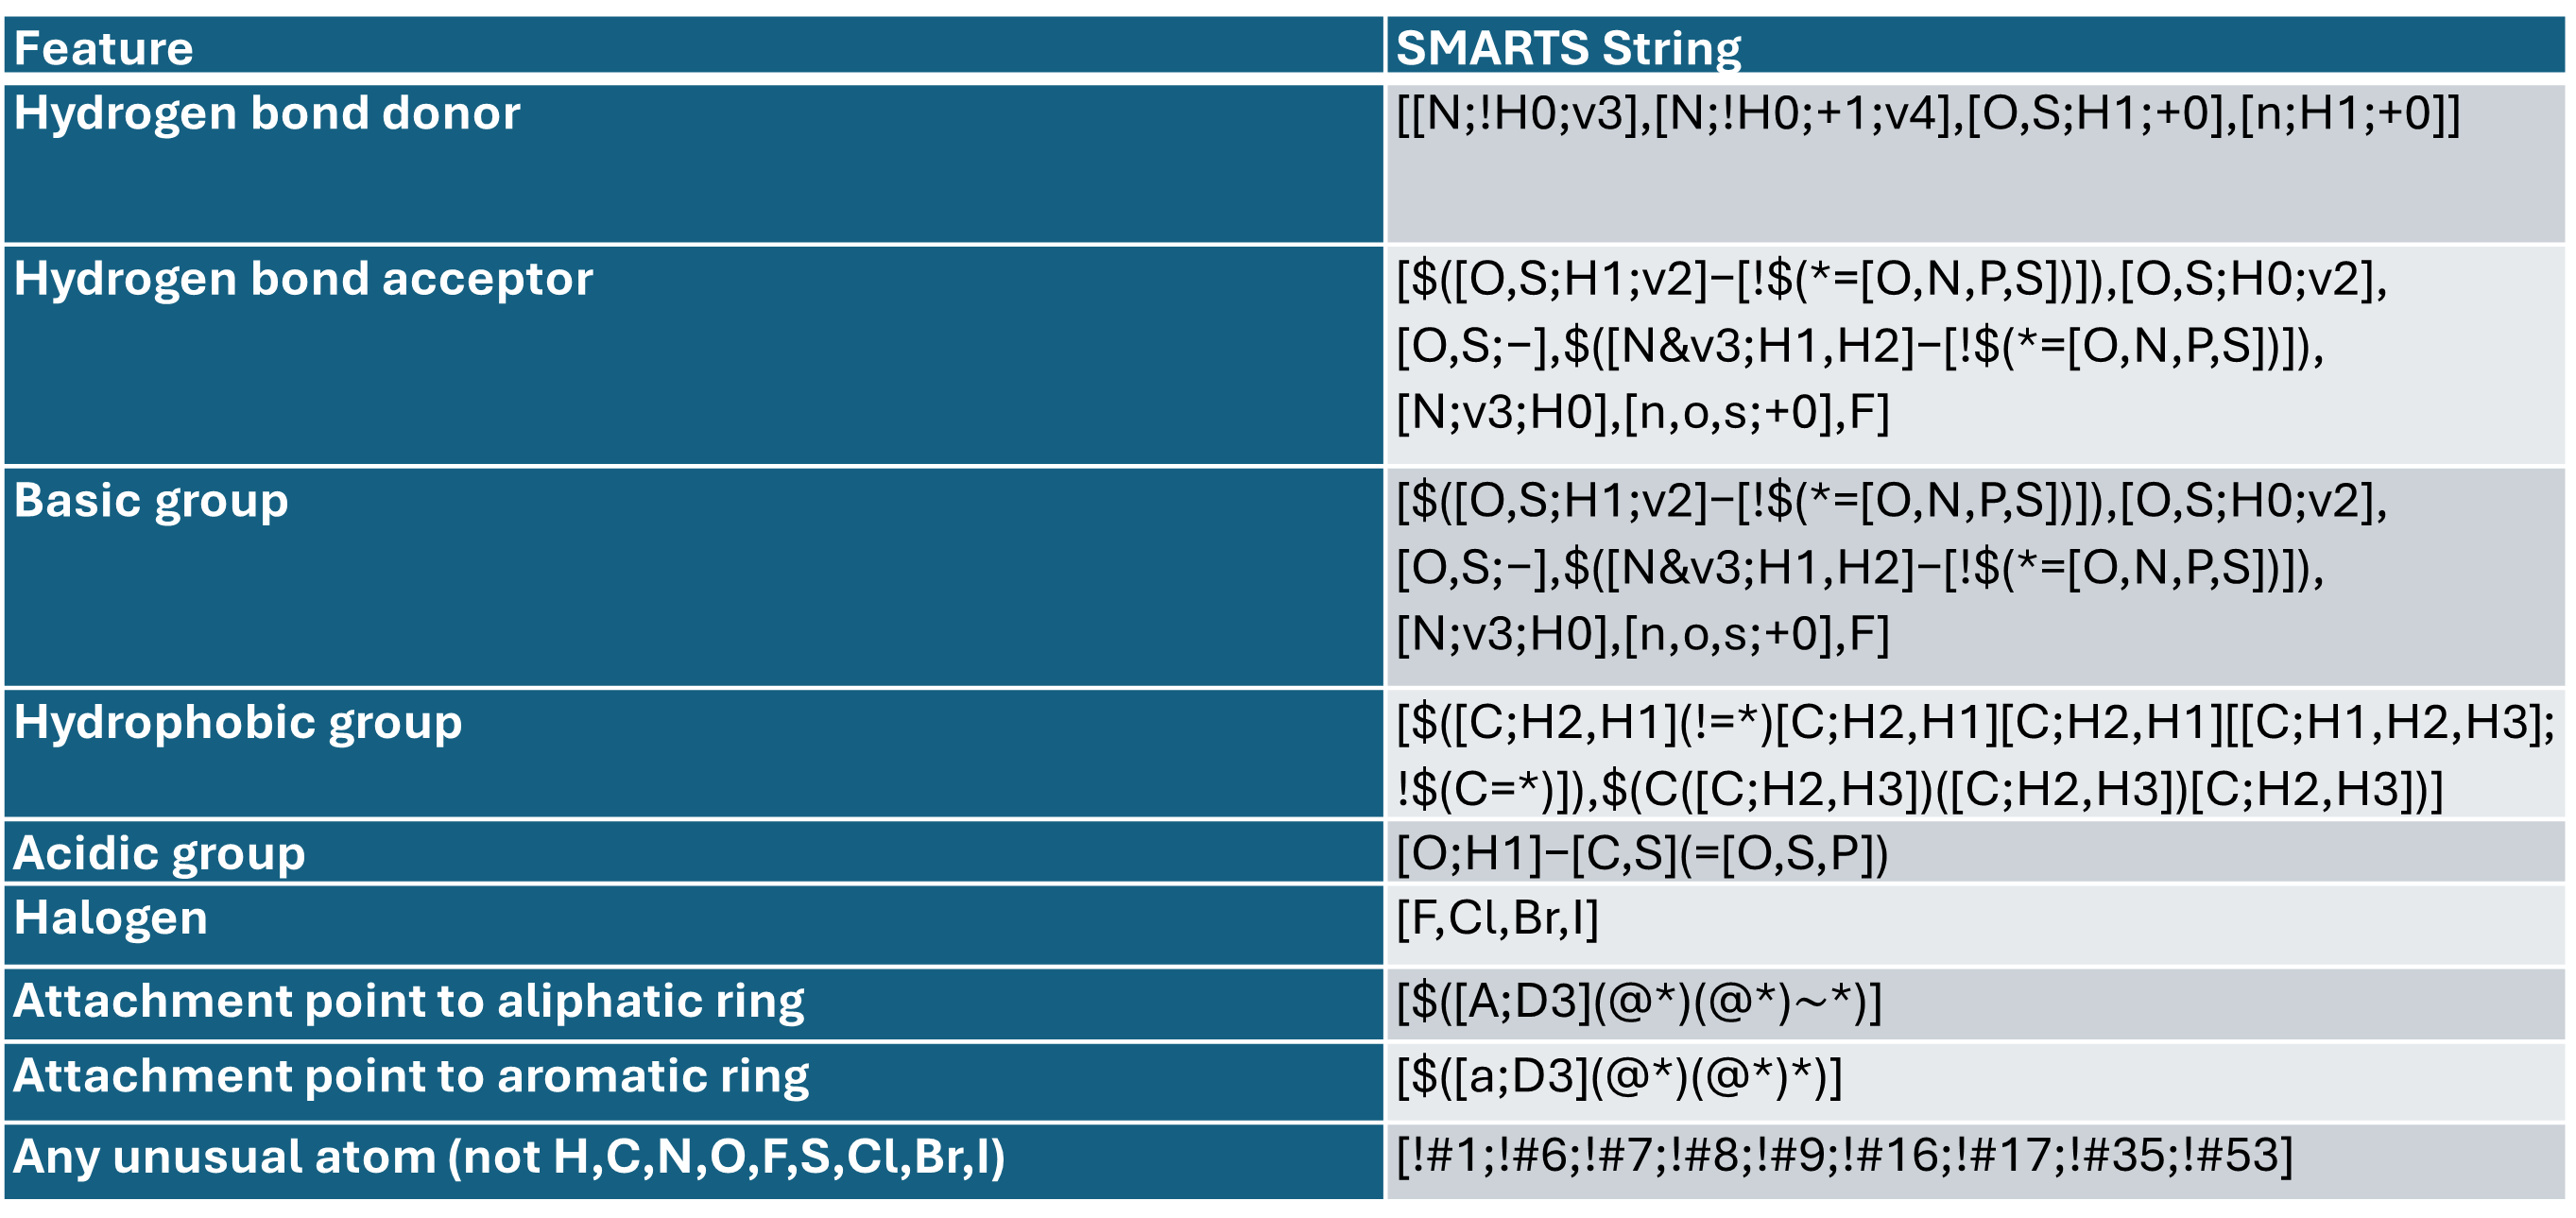
\includegraphics[width=1.05\linewidth]{gobbi_features.png}
    \caption{Features used in Gobbi / Poppinger 1999}
    \label{tab:gobbi_features}
\end{table}



\subsection{Generation of fingerprints}


In addition to the RdKit implementation, also a very simple version of the ECFP fingerprint has been implemented in Python.
This version lacks all the opimizations of the RdKit functions implemented in C, but allows for a very transparent selection of features and different hash functions can be applied.
Furthermore, it allows a custom inclusion of radii, e.g. only the substructures corresponding to the maximum radius, i.e. the more local information can discarded.
Alternatively, custom atom variants can be passed to the RdKit functions.

The feature Morgan fingerprint  uses other features which directly encompass information relevent for biological activity.
Donor, Acceptor, Aromatic, Halogen, Basic, Acidic
The corresponding SMARTS strings are shown in table \ref{tab:rdkit_featurefp_features}.


RdKit also allows to define custom invariants, i.e. one can endow each atom of the molecule with a value; given this value is identical to the values assigned to another atom, the atoms are considered isomorphic.
The effect of this invariants is visualized using 5-Ethyl-2-methylpyridine (\ref{fig:5_ethyl_2_methyl_pyridine}): One time with the full default RdKit feature set (\ref{fig:radius1_all_default_features}), with atomic number only (\ref{fig:radius1_nobonds_onlyatomnr}) , and with topological information only (\ref{fig:radius1_onlytopological}), i.e. all atoms are isomorphic to each other.

\begin{figure}
    \centering
    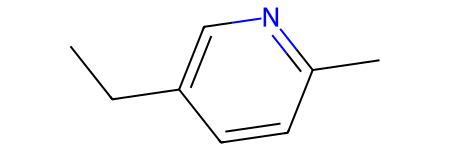
\includegraphics[width=0.75\linewidth]{5_ethyl_2_methyl_pyridine.png}
    \caption{5-ethyl-2-methyl-pyridine}
    \label{fig:5_ethyl_2_methyl_pyridine}
\end{figure}


\begin{figure}
    \centering
    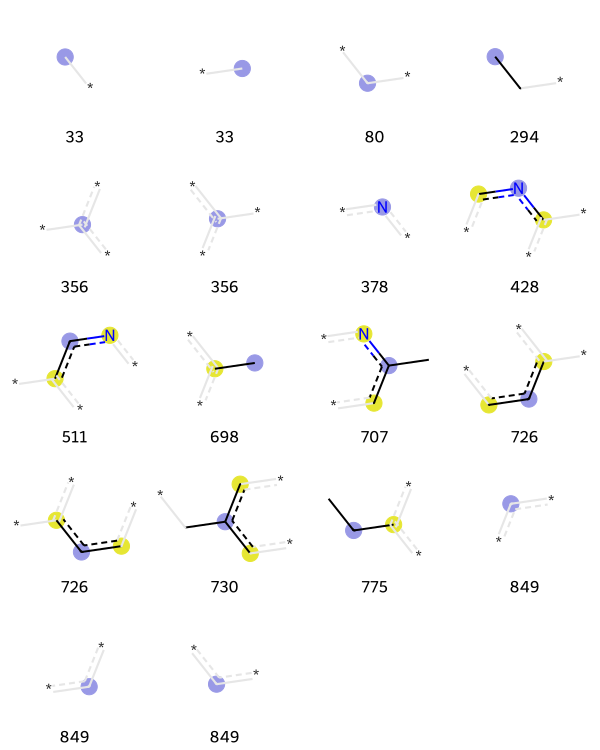
\includegraphics[width=0.75\linewidth]{radius1_all_default_features.png}
    \caption{all substructures up to radius 1; default RdKit features }
    \label{fig:radius1_all_default_features}
\end{figure}

\begin{figure}
    \centering
    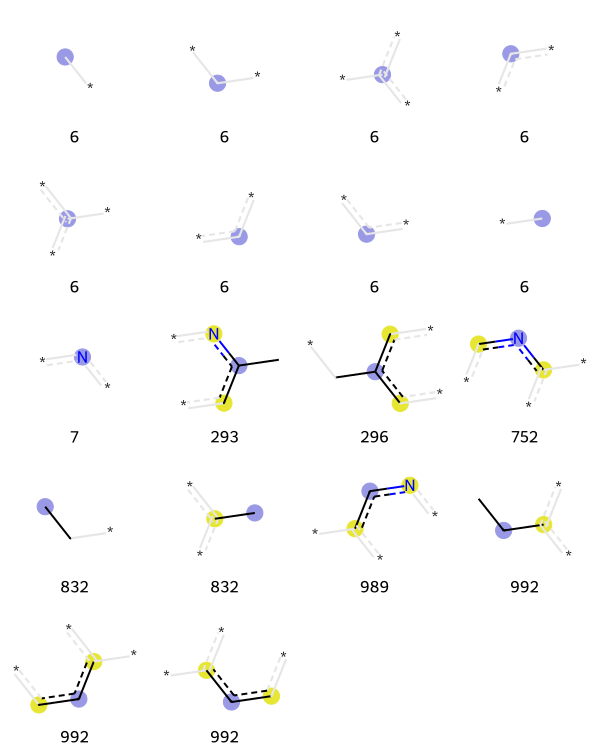
\includegraphics[width=0.75\linewidth]{radius1_nobonds_onlyatomnr.png}
    \caption{all substructures up to radius 1; only atom number as feature, without bond features }
    \label{fig:radius1_nobonds_onlyatomnr}
\end{figure}

\begin{figure}
    \centering
    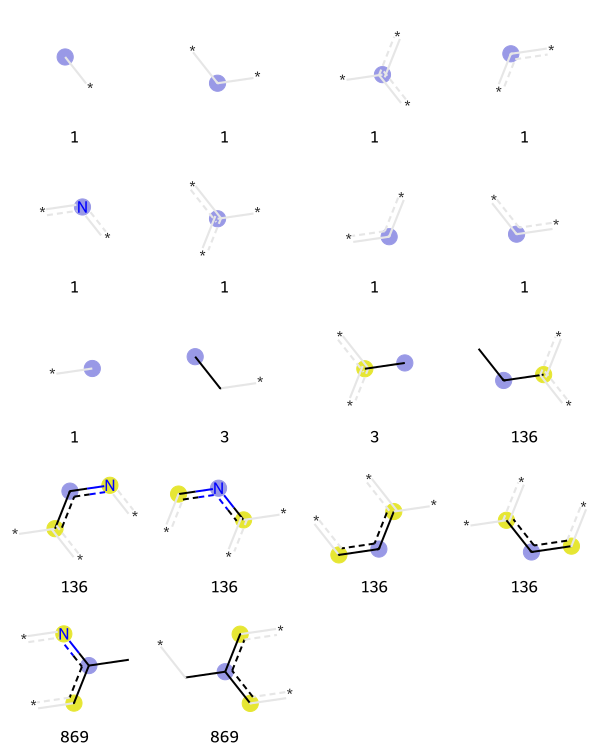
\includegraphics[width=0.75\linewidth]{radius1_onlytopological.png}
    \caption{all substructures up to radius 1; only topological information, without bond features}
    \label{fig:radius1_onlytopological}
\end{figure}

For the protein-ligand interaction task, also the physicochemical fingerprints have been used.





\subsection{Permutation of graph layers}

For assessing the information flow across multiple graph layers, the effect of permutation was studied: After the layer, the output is randomly permuted.

This permutation annihilates the permutation invariance of the graph representation; however, the values and thus statistics like the mean and variance stay the same.

Furthermore, it seems to be plausible that later permutation-invariance annihilating permutations are not that severe because at this stage, all nodes receive information from virtually all other nodes and thus the differences are minor compared to the previous layers. 

\subsection{Important features and (hyper-)parameters}

For obtaining the best hyperparameters for a specific architecture, the Optuna package has been used \cite{Akiba.25.07.2019}.
Hyperparameter optimization posed some peculiar challenges due to the complex nature of the data.
For the GNNS, the main problem is the complex interaction of graph- and classifier-part.
In principle, this could lead to misleading conclusions concerning the performance of the involved graph layers.


\subsubsection{Jumping Knowledge}

Jumping knowledge, as introduced in \cite{Xu.01.10.2018}, allows the combination of the output of the GNN layers in the final aggregation layer.
Different functions for the aggregation have been proposed: Either concatenation of all layer outputs, or the maximum can be used. Alternatively, a LSTM which subsequently processes the layer outputs can be trained.
Jumping knowledge is introduced as means to harness also more intricate, and possibly distant long-range interactions.
In \cite{Xu.01.10.2018}, networks with jumping knowledge performed superior in many tasks. In this context, it is also mentioned that a small number of layers (2) in many tasks performs better than more complex architectures.


Alternatively, one could simply concatenate the output of the individual layers, but apply different activation functions (or other transformation) on the layer-output before it is incorporated into the aggregation.
Given the fact that also ECFPs store the structures found at a smaller radius and do not discard this information, implementation of jumping knowledge or the final concatenation of the layers promises to provide a graph-based representation which is more similar.
For the experiments, also a more sophisticated approach has been implemented, applying on the copied values to be concatenated different operations, e.g. activation functions, than on the values which are processed in the subsequent graph layers (see section 'Custom activation functions').

\subsubsection{Normalization techniques}

Batch Normalization (BN) is a technique used to stabilize and speed up the training of deep neural networks by normalizing the input to each layer. It tackles the internal covariate shift, i.e. a change in the distribution of network activations  due to the change of the distribution of the parameters during training. This phenomenon, called internal covariate shift, makes training harder because the network needs to constantly adapt to these changes.
Batch normalization normalizes the input of each layer by subtracting the batch mean and dividing by the batch standard deviation:

\begin{math}
\hat{x}_i = \frac{x_i - \mu_B}{\sqrt{\sigma_B^2 + \epsilon}}
\end{math},
where $\sigma_B^2$ is the variance and $\mu_B$ the mean of the batch.

Two parameters, $\gamma$ and $\beta$, are learnt for shifting and scaling the normalized output:
\begin{math}
y_i = \gamma \hat{x}_i + \beta
\end{math}
  
On many occasions, batch normalization leads to much faster training. By normalizing the inputs, gradients become more stable, which leads to faster convergence. Furthermore, reduced sensitivity to initialization: The model is less sensitive to the choice of initial weights. Batch normalization also provides regulizarization, it introduces noise because the normalization is based on the batch, which helps prevent overfitting. By doing so, in some cases, it alleviates the need for additional dropout.
        
During inference, BN uses running averages of the mean and variance computed during training.

Layer Normalization (LN) is a similar technique, but instead of normalizing across a batch of examples, it normalizes across the features in a single layer for each data instance individually. This is useful in contexts where batch normalization does not perform well, such as for sequential data or small batch sizes, e.g. it is widely used in Transformers.


\subsubsection{Custom activation functions and binarization of output}

In Duvenaud et al. 2015 \cite{Duvenaud.30.09.2015}, it was stated that the Neural Fingerprint behaves similar to a circular fingerprint for big, random weights.
For an activation function which approximates the binary function, behaviour should therefore become more ECFP-like.

The scaled sigmoid function is defined by:

\[
\sigma_{\alpha}(x) = \frac{1}{1 + e^{-\alpha x}}
\]

and the hardtanh function:

\[
\text{Hardtanh}(x) =
\begin{cases} 
-1 & \text{if } x \leq -1 \\
x & \text{if } -1 < x < 1 \\
1 & \text{if } x \geq 1 
\end{cases}
\]



\begin{figure}
    \centering
    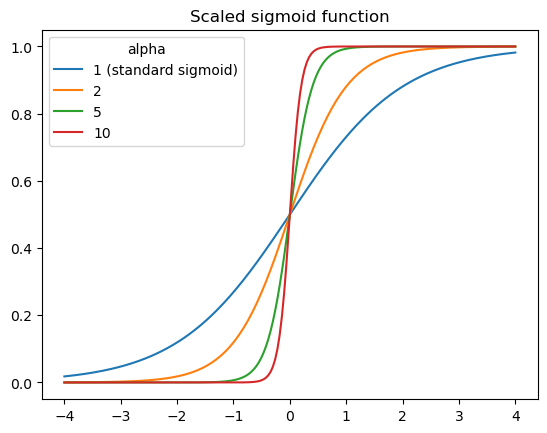
\includegraphics[width=0.5\linewidth]{scaled_sigmoid.png}
    \caption{Enter Caption}
    \label{fig:enter-label}
\end{figure}

In principle, though differentiable, such a steep activation function will lead to training difficulties on many occasions.
Therefore, it is not traced back during backpropagation.
(However, different set-ups would be possible, not only the Straight-Through Estimator.)




\[
\text{ScaledSoftmax}(x_i) = \frac{e^{\alpha x_i}}{\sum_{j=1}^{n} e^{\alpha x_j}}
\]

This allows a combination with the layer concatenation described in the section about Jumping Knowledge.


An alternative approach is the usage of binary neural networks \cite{Yuan.2023} or similar ways to achieve binary output without forgoing differentiability.

A common approach is the Straight-Through Estimator proposed by Hinton in 2012 \cite{Bengio.15.08.2013}. To retain differentiability, during backpropagation the identity function is used instead of the non-differentiable function. This gives (in particular for deep networks) a biased estimate, but was shown to be efficient in practice.



\subsubsection{Pooling and aggregation functions}

\cite{Schweidtmann.2023}

Common aggregation functions are mean, max and sum. For GINs, it has been shown that sum-aggregation has the highest expressivity in distinguishing between input graphs.
(However, it should be stressed again that this does not imply that sum-aggregation always provides the highest performance in specific tasks.)

A more sophisticated choice is Set2Set \cite{Vinyals.19.11.2015}.
This pooling operator is based on a LSTM refinement step.

\begin{align*}
q_t &= \text{LSTM}(q_{t-1}^*) \\
\alpha_{i,t} &= \text{softmax}(x_i \cdot q_t) \\
r_t &= \sum_{i=1}^N \alpha_{i,t} x_i \\
q_t^* &= q_t \, \| \, r_t
\end{align*}

In principle, one can also try to emulate fingerprint-like behaviour by deploying suitable pooling operations.
DiffPool segments the graph into smaller subgraphs using an assignment matrix.
\cite{Ying.22.06.2018}

However, it has to be kept in mind that the fingerprints create subgraphs depending on unique molecular features.

\subsection{Enhanced training strategies}

As outlined in the previous section, activity cliffs as well as the presence of dissimilar molecules in the training set are problematic for the performance of GNNs. Additionally to common methods like dropout and normalization, also a judicious selection of the loss function could improve the results.
For most runs presented, MAE was chosen since this is also mostly used in previous publications on GNNs and molecular property prediction.

Moreover, given the problem of outliers, it seems to be advisable to use a loss function robust in this regard (however, this is two-fold: on the other hand, in some cases, outliers are pair of an activity cliff and it is of great interest to figure out under which circumstances they appear).

In case of Attentive FP, the default parameters of the Pytorch Geometric model have been used.




\subsection{Combination of GNNs and global feature vector}

The potential dependency on global features gives rise to the question how global information could be incorporated into the node representation. On the other hand, perhaps a separation of both steps - i.e. GNN layers and subsequent concatenation with a global ffeature vector - could be even more promising.

In general, numerous variants are possible.
Or implement the global features as attention vector which the nodes can attend to (e.g. via the neural network within the GIN layer).



\subsection{Global feature calculation}

As a further baseline, predictions from global properties alone were computed. 
For the calculation, functions of RdKit were used.


These features include, amongst others, the accessible surface area, the number of specific atoms and the molecular weight (see table \ref{tab:molecular_properties}).

Many of these features are collinear; an appropriate subset has been used.

One could also select all global features indicating the number of occurrences of a particular element. In case that only the number of different atom types is considered, this should be equivalent to a Morgan fingerprint of radius zero and only atom type as invariant.


\begin{table}[h!]
\centering
\begin{tabular}{|l|l|}
\hline
\textbf{Property} & \textbf{Description} \\ \hline
\texttt{molecular\_weight} & The molecular weight of the compound. \\ \hline
\texttt{logP} & The partition coefficient (logP) of the compound. \\ \hline
\texttt{num\_rotatable\_bonds} & The number of rotatable bonds in the molecule. \\ \hline
\texttt{tpsa} & The topological polar surface area of the molecule. \\ \hline
\texttt{num\_h\_donors} & The number of hydrogen bond donors in the molecule. \\ \hline
\texttt{num\_h\_acceptors} & The number of hydrogen bond acceptors in the molecule. \\ \hline
\texttt{molar\_refractivity} & The molar refractivity of the molecule. \\ \hline
\texttt{fraction\_csp3} & Fraction of the molecule's carbons that are sp3-hybridized. \\ \hline
\texttt{num\_heavy\_non\_c\_atoms} & Number of heavy non-carbon atoms in the molecule. \\ \hline
\texttt{num\_carbon\_atoms} & Number of carbon atoms in the molecule. \\ \hline
\texttt{num\_non\_standard\_atoms} & Number of atoms not being C, N, O, or S. \\ \hline
\texttt{num\_nitrogen\_atoms} & Number of nitrogen atoms in the molecule. \\ \hline
\texttt{num\_oxygen\_atoms} & Number of oxygen atoms in the molecule. \\ \hline
\texttt{num\_sulphur\_atoms} & Number of sulphur atoms in the molecule. \\ \hline
\texttt{num\_rings} & Total number of rings in the molecule. \\ \hline
\texttt{num\_atoms\_in\_rings} & Number of atoms that participate in any ring. \\ \hline
\texttt{num\_atoms\_in\_two\_rings} & Number of atoms that participate in two rings. \\ \hline
\texttt{total\_num\_atoms} & Total number of atoms in the molecule. \\ \hline
\texttt{num\_single\_bonds} & Number of single bonds in the molecule. \\ \hline
\texttt{num\_double\_bonds} & Number of double bonds in the molecule. \\ \hline
\texttt{num\_triple\_bonds} & Number of triple bonds in the molecule. \\ \hline
\texttt{num\_aromatic\_bonds} & Number of aromatic bonds in the molecule. \\ \hline
\texttt{total\_num\_bonds} & Total number of bonds in the molecule. \\ \hline
\end{tabular}
\caption{Description of global molecular properties.}
\label{tab:molecular_properties}
\end{table}



\section{Differences between Graph Neural Network-based representations and Morgan fingerprints}

Again, the question whether different molecular graphs are distinguishable for a specific architecture has to be separated from the performance on a learning task.
However, the differences are a little bit more nuanced: 
At first glance, the number of layers of a (standard, i.e. non-higher order) GNN architecture resembling the radius of the Morgan Fingerprint: In the first layer, information of the neighbours is incorporated into the feature vector of each node; at the next layer, the neighbours of a specific node already contain information about the neighbours of the neighbours of this node and so information of nodes which are two edges far away is incorporated, etc.

Indeed, for radius 1, the unique entries are, as expected, identical.


The workflow of the Morgan Fingerprint suggests the processing of subgraphs: In the first iteration of the Morgan algorithm, all rooted subgraphs of radius 1 are investigated, at the next iteration of radius 2, and so on. 
A construction of all rooted subgraphs of a specific size of the molecular graph and subsequent counting of isomorphic subgraphs should give the same result as the Morgan Fingerprint (but is, due to the complexity of determining isomorphic subgraphs, computationally much more demanding), exempt for events like hash collisions.

In particular, the results in this study (presented in the next section) as well as in previous publications also show that GIN architectures do not perform equal to Morgan Fingerprints (usually, the effect of frozen layers is not investigated; however, one would not assume that freezing fully removes the differences, in particular in those cases in which GINs perform worse).

A straightforward approach for creating a neural version of a Morgan Fingerprint would thus create all subgraphs up to a given radius and then perform usual GNN operations on these subgraphs.

Nested Graphs should give a similar number of subgraphs.


For the determination of isomorphic subgraphs, the Weisfeiler-Leman algorithm as well as an exact algorithm were applied (for both, the NetworkX-library was used).
